In order to test the hypothesis, we first derive a number of subgoals/questions from the hypothesis.

Questions:
\begin{enumerate}
    \item{How important are the labels in graphs? Does structural-only data improve the classification score?}
    \item{How does the classification performance compare to classical, non-structural approaches?}
    \item{How does the size of a graph affect the classification result?}
\end{enumerate}

\paragraph{Question: ``How similar/diverse are the graphs structurally?"}
If the structure of the graphs is too similar and the structural differences are not distinct between the classes, they most likely will not be that useful for classification.
When comparing the graph similarity with respect to some graph kernel, the graphs in some class should be distinguishable from the graphs in another class.

To explore the differences, we look at three questions in particular:
``How similar are the graphs... $a)$ in the same class, $b)$ between (pairs of) classes and $c)$ in the complete dataset?"

\todo{Since we are especially interested in answering structure-related questions about the graphs, we first have to distinguish structural from non-structural data.}
\todo{Explain the used metrics and how they relate to hypothesis}
\todo{Explain the datasets and how they differ, why they are important?}
\todo{Introduce the baselines, explain how they relate to the hypothesis, why they - are chosen, how they differ}
\todo{Explain methodology, why the chosen metric really captures the problem at - hand}
\todo{Work out differences of graph types, find similarities across datasets}
\todo{Provide the questions that are relevant for the hypothesis}
\todo{Answer these questions through metrics/results}

\refsubsection{Experiments}{subsec:experiments}
\todo{Test the hypothesis}
\todo{Tables with results}
\todo{Mention difficulties and possible solutions}
\todo{Add runtime analysis}

\subsubsection{Baselines}

\paragraph{Text-based}
\todo{Preprocessing}
\todo{CountVectorizer, TfIdfVectorizer}

\paragraph{Graph-based}
\todo{Preprocessing}
\todo{Window sizes}
\todo{}

\subsubsection{Approach}
\todo{Combined}
\todo{Code by Tobias, explain steps}

\begin{figure}[h]
\centering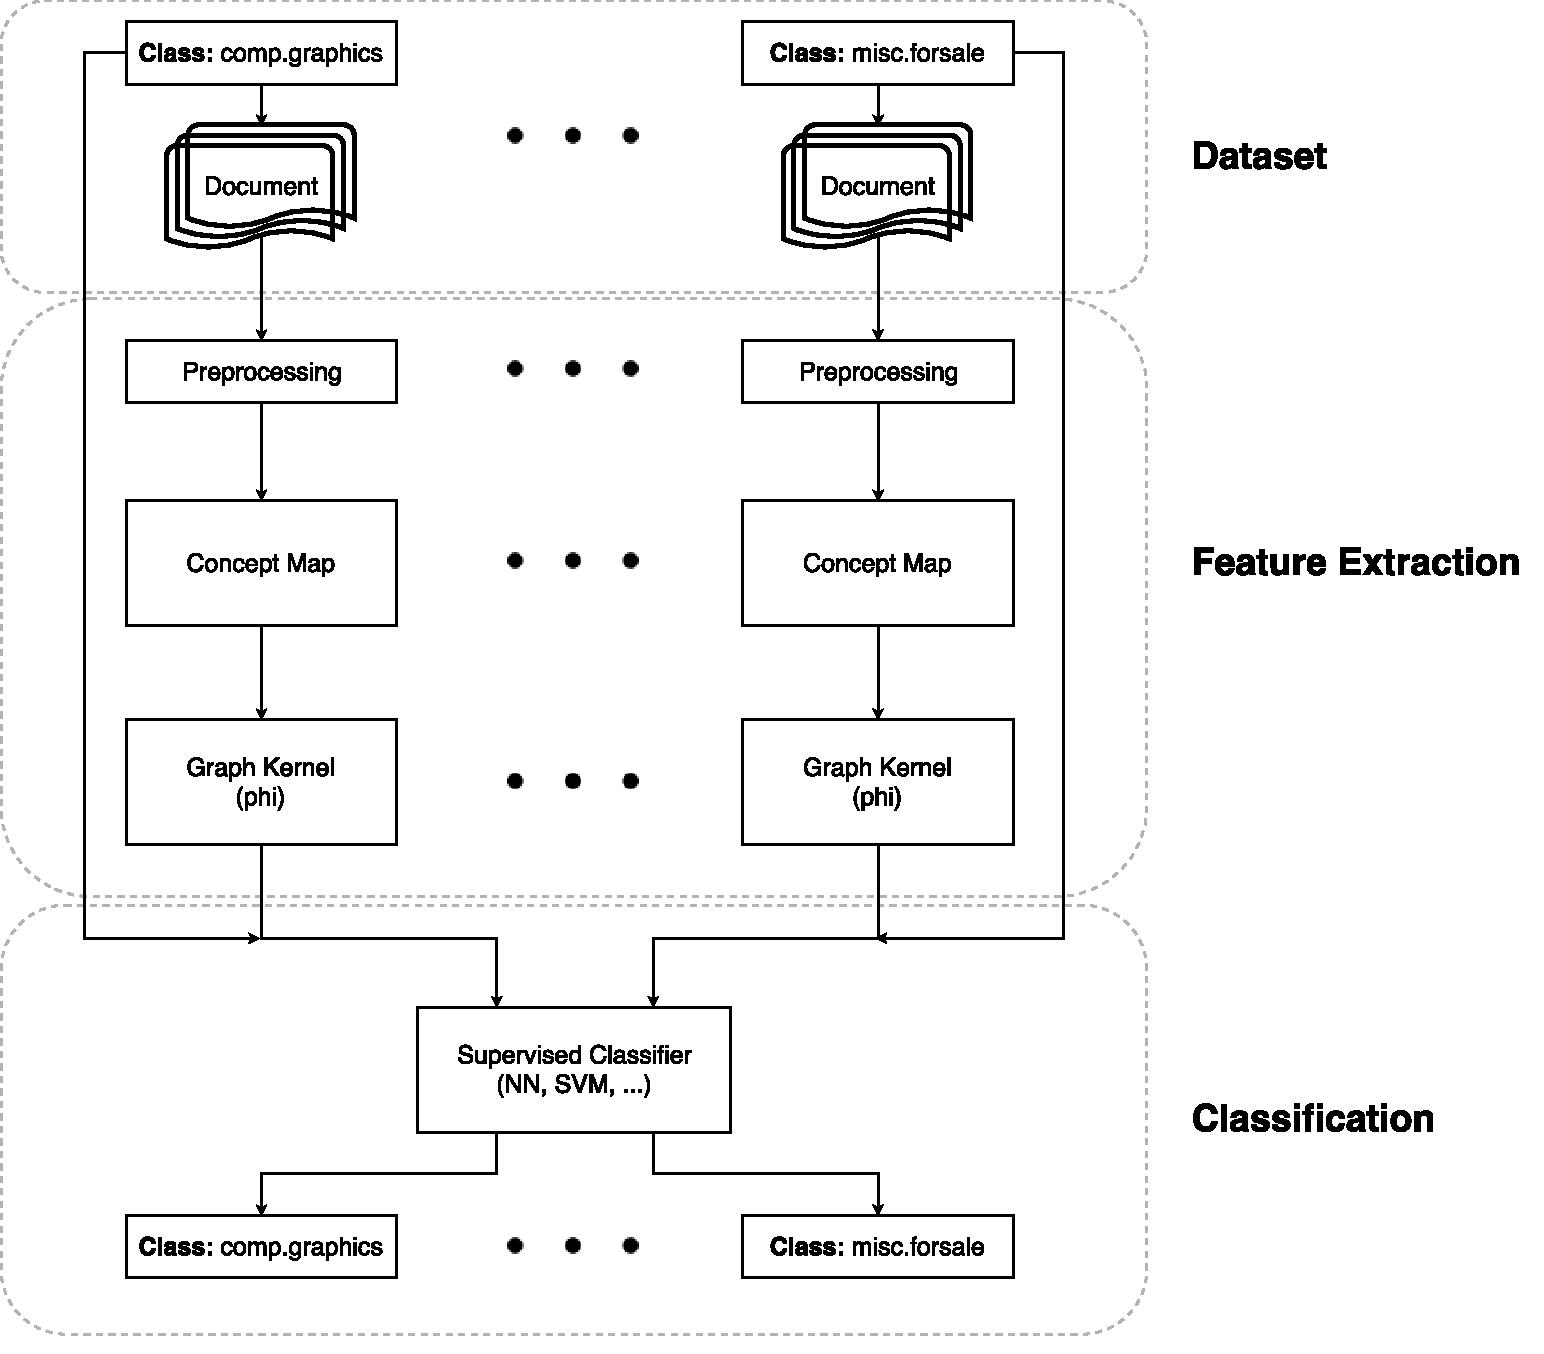
\includegraphics[width=0.6\linewidth]{assets/figures/approach.pdf}
\caption{\todo{Caption}}
\end{figure}

\refsubsection{Datasets}{subsec:datasets}
\todo{Statistics about datasets and derived graphs}
\todo{Skewed classes}
\todo{Graph statistics}
\todo{Give hints where to download the datasets from}

\begin{figure}
\centering
\begin{tabular}{lrr}

dataset &  \# classes &  \# documents \\
\midrule
ling-spam       &  2 &  2893 \\
ng20            &  20 &  18846 \\
r8              &  8 &  9459 \\
reuters-21578   &  90 &  13328 \\
review\_polarity &  2 &  2000 \\
rotten\_imdb     &  2 &  10000 \\
tagmynews       &  7 &  32600 \\
webkb           &  7 &  8274 \\

\end{tabular}

\caption{Datasets}
\end{figure}

\refsubsection{Methods}{subsec:methods}
\todo{Combined}
\todo{Scaler}
\todo{Merging nodes?}

\subsubsection{Cross-Validation}

\subsubsection{Pre-Processing}

\subsubsection{Metrics}

\subsubsection{Significance tests}

\refsubsection{Implementation}{sec:implementation}
\todo{Scikit-learn, networkx, \dots}
\todo{Code by Tobias to extract concept maps}
